\myChapter{Grundlagen}\label{chap:basics}
Im folgenden Kapitel sollen einige wichtige Grundbegriffe und Technologien
eingeführt werden, die für das weitere Verständnis der Arbeit wichtig sind. Neben
der Festlegung der verwendeten Begriffe wird die Java Plattform und die dort
verwendeten Technologien näher behandelt. Anschließend wird das Konzept des
\ac{RPC} eingeführt und verschiedene Austauschformate für die Übertragung von
Daten in einem Netzwerk erläutert.

Vom Leser werden Kenntnisse in der \emph{Objektorientierten Programmierung} und
der dabei verwendeten Terminologie sowie Grundkenntnisse über häufig verwendete
\emph{Design Patterns} (siehe \cite{gof} und \cite{fowler:2002}) erwartet. Da die
Implementierung in Java und einer Java sehr ähnlichen Programmiersprache
erfolgte, sind gute Java Kenntnisse ebenfalls empfehlenswert. Auch von Grundlagen in
Netzwerken, einschließlich grundlegender Web Technologien, wird ausgegangen.

\section{Begriffe}

\begin{description}
\item[Framework]\label{define:framework} Ein Framework ist in der
objektorientierten Programmierung eine Sammlung von Klassen, welche - meist unter
der Verwendung verschiedener Design Patterns - einen Rahmen für die Architektur
einer Anwendung bieten. Im Unterschied dazu stellt eine Klassenbibliothek
lediglich eine Reihe von Klassen bereit, die von einem Entwickler verwendet
werden können.
\item[Benutzer]\label{define:benutzer} Die folgenden Kapitel beziehen sich auf
den Aufbau einer Schichtenarchitektur. Deshalb soll sich in diesem Zusammenhang
der Begriff Benutzer immer auf die jeweils übergeordnete Schicht beziehen. Aus
Sicht eines Frameworks oder einer Klassenbibliothek ist der Benutzer der Teil
einer Anwendung, der diese verwendet. Ein menschlicher Benutzer soll im weiteren
Verlauf als Anwender bezeichnet werden.
\item[Assoziatives Array]\label{define:assocarray} Assoziative Arrays\footnote{In
verschiedenen Programmiersprachen auch Dictionary, Hash oder Map genannt}
erlauben die Adressierung von Datenelementen über beliebige, eindeutige
Schlüssel (siehe \cite{wiki:assocarray}). Die dafür benötigte Schnittstelle
umfasst dabei die Operationen \emph{get(key)}, \emph{put(key, value)} und
\emph{remove(key)}. Da assoziative Arrays von den meisten Programmiersprachen
unterstützt werden, stellen sie eine wichtige Grundlage für den Austausch
strukturierter Daten dar. Auch im weiteren Verlauf dieser Arbeit wird das Konzept
der assoziativen Arrays wiederholt aufgegriffen. Beispiele hierfür sind:
\begin{itemize}
  \item Java Maps und JavaBeans (in Kapitel \ref{subsec:javabeans})
  \item NoSQL Datenbanken (in Kapitel \ref{sec:datasource})
  \item JSON und XML (in Kapitel \ref{subsec:assocequ})
  \item Anwendungscaches (in Kapitel \ref{service:cache})
  \item Java Property Dateien (in Kapitel \ref{service:i18n})
\end{itemize}
\item[Verteilt vs. Netzwerk-basiert]\label{define:networkbased} Die Literatur
(vgl. \cite{fielding:2000} S. 24) unterscheidet zwischen verteilten und
netzwerkbasierten Systemen. Ein verteiltes System verhält sich gegenüber dem
Benutzer wie ein lokales System, wird aber auf mehreren CPUs ausgeführt. Im
Gegensatz dazu kommuniziert ein netzwerkbasiertes System zwar über ein Netzwerk,
muss dies aber nicht unbedingt für den Benutzer transparent übernehmen. Der
Schwerpunkt dieser Arbeit soll auf netzwerkbasierten Systemen liegen.
\end{description}

\section{Java Plattform}
Die \ac{JVM} stellt eine Middleware dar, die die platt\-form\-unabhängige
Ausführung von in entsprechendem Bytecode vorliegenden Programmen ermöglicht (vgl.
\cite{wiki:jvm}). Die \ac{JVM} ist ein Teil des \ac{JRE} und stellt zusammen mit
einer großen Anzahl an Klassenbibliotheken die Java Plattform.

\subsection{Programmiersprachen für die JVM}
Zur Einführung der \ac{JVM} in der Version 1.0 gab es nur
einen Bytecode Compiler für die Programmiersprache Java. Mit steigender
Verbreitung der Plattform und besserer Performance der \ac{JVM} wurde es
zunehmend interessant, auch andere Programmiersprachen in auf der \ac{JVM}
lauffähigen Bytecode zu übersetzen. Man kann somit unter anderem
Programmiersprachen, für die bisher nur Compiler für spezielle Plattformen
existierten, eine plattformunabhängige Ausführungsumgebung zur Verfügung
stellen oder interpretierte Programmiersprachen durch die Kompilierung in Java
Bytecode performanter ausführen, ohne dass die Portabilität verloren geht.

\subsubsection{Unterschiedliche Lösungsansätze}
Ein weiteres aktuelles Thema bei Programmiersprachen für die \ac{JVM} ist die
Möglichkeit, durch bestimmte Spracheigenschaften Probleme einfacher und
effektiver angehen zu können als es mit Java selbst der Fall ist. So übernehmen
einige Sprachen wie Scala\footnote{Scala steht für \emph{Scalable Language}} oder
Clojure Ansätze aus der funktionalen Programmierung. Dadurch kann unter anderem
die Komplexität und Fehleranfälligkeit der nebenläufigen Programmierung
reduziert werden, da es, anders als in objektorientierten Programmiersprachen,
keinen globalen Zustand gibt, auf den Datenzugriffe aus verschiedenen Threads
synchronisiert werden müssen. Auch für die meisten populären dynamischen und
interpretierten Sprachen gibt es inzwischen Implementierungen für die \ac{JVM}.
Tabelle \ref{tab:jvmlangs} zeigt eine Übersicht über einige auf der \ac{JVM}
lauffähigen Programmiersprachen.

\begin{table}[h] \begin{tabularx}{\textwidth}{llX} \toprule
   \tableheadline{Name} & \tableheadline{Bemerkung} & \tableheadline{URL} \\
   \midrule
   		Java & Erste Sprache, OOP & \url{http://java.sun.com} \\
    	Groovy & Dynamisch, OOP & \url{http://groovy.codehaus.org/}
    	\\ Scala & OOP / Funktional Hybrid & \url{http://www.scala-lang.org/} \\
    	Clojure & Funktional & \url{http://clojure.org/} \\
    \midrule
    	JRuby & Ruby & \url{http://jruby.org} \\
    	Jython & Python & \url{http://jython.org} \\
    	Rhino & JavaScript & \url{http://mozilla.org/rhino/} \\
	\bottomrule
	\end{tabularx}
	\captionof{table}[Programmiersprachen für die JVM]{Auswahl einiger
	Programmiersprachen f\"ur die JVM\footnotemark}
	\label{tab:jvmlangs}
\end{table}
\footnotetext{Quelle: \cite{wiki:jvmlanguages}}

\subsubsection{Groovy}
Eine dieser "`neuen" \ Programmiersprachen, die direkt für die \ac{JVM}
entwickelt wurden, ist Groovy\footnote{\url{http://groovy.codehaus.org/}}. Es
handelt sich hierbei um eine dynamische, objektorientierte Sprache, die Einflüsse aus
Programmiersprachen wie Python, Ruby und SmallTalk für Java Entwickler in einer
an Java angelehnten Syntax verfügbar macht (siehe \cite{koenig:2007}). Dies
bedeutet auch, dass der Großteil eines Java Quelltextes gleichzeitig valide
Groovy Syntax ist. Dabei besitzt Groovy aber einige zusätzliche Merkmale:

\begin{description}
  \item[Dynamische und statische Typisierung] Dynamische Typisierung bedeutet,
  dass der Typ einer Variable zur Laufzeit von deren Wert abhängt. Im Gegensatz
  dazu wird bei der statischen Typisierung der Typ einer Variable zum Zeitpunkt
  der Kompilierung festgelegt und kann nur entsprechende Werte annehmen. Groovy
  unterstützt beide Möglichkeiten, wodurch das jeweils passende Typsystem
  verwendet werden kann; die statische Typisierung erfolgt identisch mit der in
  Java. Neben der dynamischen Typisierung erlaubt es Groovy auch, zur Laufzeit
  neue Methodendefinitionen zu einer Klasse hinzuzufügen oder existierende
  Definitionen zu ändern.
  \item[Java Integration] Einer der größten Vorteile von Groovy
  gegenüber anderen Sprachen für die \ac{JVM} ist die nahtlose Integration mit
  einer bereits existierenden Java Codebasis. Da Groovy ebenfalls in Java
  Bytecode kompiliert wird, ist eine natürliche Verwendung von Groovy Klassen
  in Java ebenso problemlos möglich wie im umgekehrten Fall.
  \item[Collections] Die Syntax von Groovy sieht eine native Unterstützung für
  Java Collections vor. Zudem wurden die Java Collection Klassen um eine Reihe
  nützlicher Methoden erweitert.
  \item[Closures] Eine Closure ist in Groovy ein anonymer
  Codeblock\footnote{Vergleichbar mit inneren anonymen Klassen in Java}, dem auch
  eine Reihe von Parametern übergeben werden können\footnote{Ist kein Parameter
  angegeben, besitzt eine Closure immer ein implizites Parameter mit dem Namen
  \emph{it}}. Sie kann auch für die Ausführung an einer anderen Stelle
  einer Variablen zugewiesen werden.
  \item[Operator Overloading] Groovy erlaubt das bisher nicht von Java
  unterstützte Überladen von Operatoren.
  \item[String Erweiterungen] Die Unterstützung für Strings wurde in Groovy
  erweitert. So ist die Referenzierung von Variablennamen in einem String
  möglich, wodurch die oft unübersichtliche Konkatenation über den + Operator
  entfällt. Auch Regular Expressions sind ein nativer Bestandteil der Groovy
  Syntax.
\end{description}

Aufgrund dieser Eigenschaften eignet sich Groovy vor allem sehr gut für die agile
Entwicklung von Anwendungen, da viele Probleme mit einem Bruchteil des
Quelltextumfangs gelöst werden können, der in Java nötig wäre. Listing
\ref{lst:groovy} zeigt ein Beispiel eines Groovy Unit Tests mit der Verwendung
von Closures, Collections und Groovy Strings. Es ist zu beachten, dass dynamische
Sprachen, also auch Groovy, grundsätzlich nicht so performant arbeiten, wie
statisch getypte Sprachen. Durch die gute Integration von Groovy und Java ist es
aber möglich, die Teile einer Anwendung in Java zu implementieren, die
performant arbeiten müssen und auf Groovy zurückzugreifen, wenn die Entwicklung beschleunigt
und vereinfacht werden soll. Von dieser Möglichkeit wurde auch bei
einigen Implementierungen Gebrauch gemacht, die in dieser Arbeit vorgestellt
werden sollen.

\pagebreak
\lstset{language=java}
\lstinputlisting[caption=Beispiel eines Groovy Unit Tests,
label=lst:groovy]{sources/groovyexample.groovy}

\subsection{JavaBeans}\label{subsec:javabeans}
JavaBeans sind wiederverwendbare Software-Komponenten für Java. Wichtigster
Kernpunkt der JavaBean Spezifikation (siehe \cite{hamilton:1997}) sind eine Reihe
von Konventionen für die Implementierung von Java Klassen, wodurch diese einfach
zu instanziieren sind und leicht in ein übertragbares (serialisierbares) Format
gebracht werden können. Damit eine Klasse als JavaBean gilt, muss sie die
folgenden Eigenschaften erfüllen (Listing \ref{lst:javabean} zeigt
ein Beispiel für ein JavaBean):

\begin{description}
\item[Default Constructor] Die Klasse muss einen öffentlichen Standardkonstruktor
definieren. 
\item[Properties] In der Objektorientierten Programmierung ist es üblich, dass
die Membervariablen einer Klasse nicht nach außen hin sichtbar sind. Für den
Zugriff von außen werden deshalb sogenannte \emph{Zugriffsmethoden (Accessor
Methods)} implementiert. Dadurch wird die Kapselung der Membervariablen
sichergestellt und der Zugriff darauf kann flexibler gestaltet werden. Für die
Definition von Zugriffsmethoden sieht die JavaBean Spezifikation eine spezielle
Namenskonvention vor. Um eine Eigenschaft zu lesen wird eine Methode nach dem
Schema \emph{Typ~getName()} definiert. Für Eigenschaften mit einem boolschen Wert
gilt die Signatur \emph{Boolean~isName()}. \emph{Name} ist hier der Name der
Eigenschaft, und beginnt immer mit einem Großbuchstaben. Zurückgeliefert wird
eine Instanz vom Typ dieser Eigenschaft. Für den schreibenden Zugriff muss eine
Methode mit der Signatur \emph{void~setName(Typ~argument)} angelegt werden. Der
Parameter argument ist dabei die zu schreibende Eigenschaft. Durch
diese Namenskonventionen werden lesende Zugriffsmethoden auch \emph{Getter-} und
schreibende Zugriffsmethoden auch \emph{Setter-Methoden} genannt. Eigenschaften,
die nur eine Zugriffsmethode für den lesenden Zugriff, besitzen werden
\emph{Read-Only} Eigenschaften genannt. Für den selteneren Fall, dass eine
Eigenschaft lediglich eine Setter Methode besitzt, nennt man diese
\emph{Write-Only} Eigenschaft.
\item[Serializable] Eine JavaBean Klasse muss das \emph{Serializable} Interface
der Java Standardbibliothek implementieren. Es handelt sich hierbei um ein
\emph{Marker Interface}, das keinerlei Methoden bereitstellt, sondern eine Klasse
lediglich auf eine bestimmte Eigenschaft hin kennzeichnet. In diesem Fall
kennzeichnet das \emph{Serializable} Interface, dass der Zustand einer Instanz
der implementierenden Klasse auch außerhalb des aktuell ausgeführten Programms
dargestellt und auch ohne Informationsverlust von dort wieder hergestellt werden
kann. Durch diese Eigenschaft können JavaBeans problemlos in Dateien gespeichert
oder über ein Netzwerk übertragen werden.
\end{description}

\lstset{language=Java}
\lstinputlisting[caption=Beispiel einer JavaBean Klasse, label=lst:javabean]
{sources/javabeanexample.java}

Da der Zugriff auf die \emph{Properties} eines JavaBean durch den jeweiligen
Namen erfolgt, können JavaBeans auch als statisches assoziatives Array angesehen
werden. Der Name einer Eigenschaft ist der eindeutige Schlüssel und die Menge der
möglichen Schlüssel sind die Namen aller Eigenschaften.

\subsection{Reflection}
Die \emph{Java Reflection API} (siehe \cite{sun:reflection}) bietet die
Möglichkeit, zur Laufzeit Informationen über Methoden und Datenmember von
Klassen und Objekten einzuholen. Dadurch ist es möglich Instanzen, von Objekten
zu erstellen und Methoden aufzurufen, die erst zur Laufzeit des Programms bekannt
sind. Vor allem Frameworks, die über Module erweitert werden können, machen von
dieser Möglichkeit häufig Gebrauch. Die Verwendung von Reflection ist
grundsätzlich langsamer als eine direkte Ausführung, da Membervariablen und
Methoden über Strings angesprochen werden und das entsprechende Aufrufziel
deshalb erst aus den Metainformationen der Java Klasse bestimmt werden muss
(vgl. \cite{wiki:reflection}).

Durch die in Kapitel \ref{subsec:javabeans} vorgestellten Namenskonventionen
können JavaBeans ebenfalls direkt durch die Reflection API verwendeten werden.
Das ist vor allem für Bibliotheken sinnvoll, die allgemein mit JavaBeans
arbeiten, ohne diese bereits zu kennen. Die \emph{Apache Commons
Beanutils}\footnote{\url{http://commons.apache.org/beanutils/}} Bibliothek bietet
hierfür eine Reihe nützlicher Klassen an.

\subsection{Spring Framework}\label{subsec:springframework}
Das Spring Framework\footnote{\url{http://springframework.org}} ist ein Open
Source Anwendungsframework für die Java Plattform zur Entwicklung von
Unternehmensanwendungen. Die bisher für diesen Zweck eingesetzte \ac{J2EE} hatte
mit der Zeit eine schwer zu handhabende Komplexität entwickelt, die vor allem bei
Entwicklungsbeginn hohe Einstiegshürden legt. Eines der Ziele des Spring
Frameworks ist, diese Entwicklung zu vereinfachen, wobei es als Alternative
oder zur Ergänzung der \ac{J2EE} verwendet werden kann. Das Spring Framework ist
in verschiedene Module unterteilt, die in Form einer Schichtenarchitektur
aufgebaut sind (siehe Abbildung \ref{ill:springmodules}).

\begin{figure}[bth]
    \center{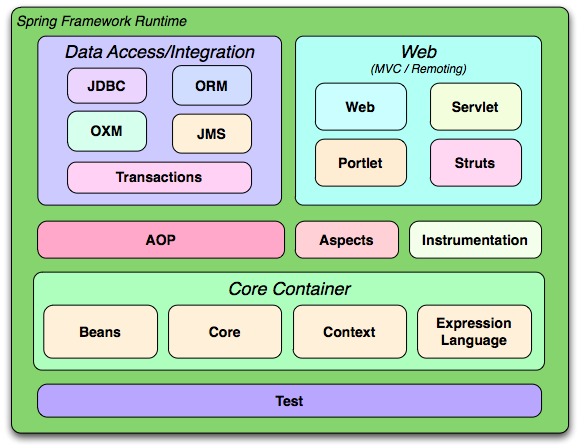
\includegraphics[width=\linewidth]{images/spring-overview.png}}
	\captionof{figure}[Spring Framework Übersicht]{Spring Framework
	Übersicht\footnotemark}
	\label{ill:springmodules}
\end{figure}
\footnotetext{Quelle: \cite{spring:reference}}

\subsubsection{Dependency Injection}
Dependency Injection befasst sich mit der grundlegenden Frage, wie man aus einem
objektorientierten Klassenmodell die in einer Anwendung benötigten Objekte und
deren Abhängigkeiten erstellen kann. Die Bereitstellung eines Dependency
Injection Containers ist eine der wichtigsten Aufgaben der Kernkomponenten des
Spring Frameworks.

Ein bisher üblicher Ansatz für die Instanziierung der benötigten Objekte ist der
des \emph{Factory} Design Patterns. Dort werden die benötigten
Konfigurationseinstellungen, oft aus verschiedenen Quellen, gelesen und die
entsprechenden Objekte instanziiert, die sich ein Benutzer dann von der Factory
holen kann. Ein Nachteil des Factory Patterns ist, dass die gesamte Umsetzung dem
Entwickler selbst überlassen ist. Damit ergeben sich zwar viele Freiheiten, da
aber eine allgemeine Konvention für die Implementierung fehlt, können auch sehr
unflexible Lösungen entstehen. Ein Problem, das dabei häufig auftritt, sind
unnötige Abhängigkeiten zwischen Objekten und Klassen, die sich mit ihrer eigenen
Instanziierung befassen müssen. Hinzu kommt, dass sich zwar inzwischen die
Auszeichnungssprache \ac{XML} als Format für Konfigurationsdateien etabliert hat,
die einzelnen Dateien in den meisten Fällen aber individuell strukturiert sind.

Im Rahmen des Spring Framework wird für Dependency Injection auch der Begriff
\ac{IOC} verwendet. \ac{IOC} bedeutet bei der Verwendung eines Frameworks, dass
sich nicht mehr der Benutzer, sondern das Framework mit der Instanziierung der
erstellten Klassen befasst. Inzwischen hat sich aber die von Fowler in
\cite{fowler:2004} geprägte und treffende Bezeichnung Dependency Injection
durchgesetzt. Für die Definition von Objekten und deren Abhängigkeiten wird eine
standardisierte \ac{XML} Konfigurationsdatei verwendet. Diese Konfiguration wird
von dem \emph{Dependency Injection Container} gelesen, der dann mittels
Reflection die dort beschriebenen Objekte instanziiert. Die Konfigurationsdatei
wird
\emph{Context} und die daraus erstellte Objektstruktur \emph{Application Context}
genannt. Die Klassen, die in einem Spring Context instanziiert werden, müssen
lediglich der schon bei JavaBeans üblichen Konvention der \emph{Properties}
folgen, also entsprechende Getter und Setter Methoden bereitstellen. Für eine so
definierte Klasse wird auch oft der Begriff \ac{POJO} verwendet, da es sich im
Grunde um eine einfache Java Klasse handelt, die lediglich gewisse Konventionen
einhält.

Bei der Entwicklung in Java ist es üblich, die Beschreibung einer Schnittstelle
durch die Definition eines \emph{Java Interface} von der eigentlichen
Implementierung zu trennen. Dadurch können andere Implementierungen verwendet
werden, ohne dass die Benutzer des Interface davon Kenntnis benötigen. In
Verbindung mit Dependency Injection wird die Verwendung von Interfaces
vollständig transparent gestaltet, da die Instanziierung der passenden
Implementierung in der Context Definition, also vollständig unabhängig von dem
Objektmodell der Anwendung, vorgenommen wird. Ein vollständiges Beispiel zur
Verwendung von Dependency Injection in Spring ist in Anhang \ref{chap:appendix}
zu finden.

\subsubsection{Aspektorientierte Programmierung}\label{define:aop}
\ac{AOP} ergänzt die objektorientierte Programmierung um einen anderen Ansatz zur
Modularisierung der Anwendungslogik (vgl. \cite{spring:reference} Abschnitt 7.1).
In der objektorientierten Programmierung wird die Anwendungslogik in einzelne
Klassen unterteilt, die Datenelemente und Methoden besitzen. Im Gegensatz dazu
ist das Konzept der aspektorientierten Programmierung die Unterteilung in
\emph{Aspekte}, die sogenannte \emph{Cross Cutting Concerns} repräsentieren.
Dabei handelt es sich um Funktionalitäten, die nicht direkt einer einzelnen
Klasse zugeordnet werden können.

Das ist beispielsweise der Fall, wenn die verschiedenen Methodenaufrufe einer
Anwendung protokolliert werden sollen. In der klassischen objektorientierten
Programmierung muss zu diesem Zweck in jeder Methode der für die Protokollierung
notwendige Aufruf eingefügt werden. Mit der Erweiterung der aspektorientierten
Programmierung ist es nun möglich, den Aspekt der Protokollierung von
Methodenaufrufen an einer zentralen Stelle, beispielsweise in einer eigenen
Klasse, zu definieren. Anschließend wird dieser Aspekt als \emph{Advice} in die
Aufrufhierarchie der betroffenen Methoden eingefügt. Dadurch wird der
Methodenaufruf an einer festgelegten Stelle unterbrochen und der an dieser
Stelle eingefügte Advice ausgeführt. Der Advice kann nun entscheiden, ob der
Methodenaufruf weiter ausgeführt werden soll oder nicht. Das Spring Framework
unterscheidet vier verschiedene Advice Typen (vgl. \cite{spring:reference}
Abschnitt 7.1.1):

\begin{description}
  \item[Before] Ein Before Advice wird vor einem Methodenaufruf ausgeführt und
  kann die Methodenausführung nicht unterbrechen.
  \item[After Returning] Kehrt eine Methode ohne Fehler zum Aufrufer zurück,
  wird der After Returning Advice aufgerufen.
  \item[After Throwing] Der After Throwing Advice wird aufgerufen, wenn die
  betroffene Methode eine Exception wirft.
  \item[Around] Der Around Advice kann Operationen vor und nach dem Aufruf
  einer Methode ausführen und außerdem entscheiden, ob der eigentliche
  Methodenaufruf weiter ausgeführt wird oder nicht.
\end{description}

Um einen Advice entsprechend ausführen zu können, erstellt das Spring Framework
ein sogenanntes \emph{Proxy} Objekt, das zwischen dem Aufrufer und dem
\emph{Zielobjekt} vermittelt. Für den Aufrufer verhält sich das Proxy Objekt wie
das eigentliche Zielobjekt. Der Unterschied bei einem Methodenaufruf soll in
Abbildung \ref{ill:aopproxy} verdeutlicht werden.

\begin{figure}[bth]
    \center{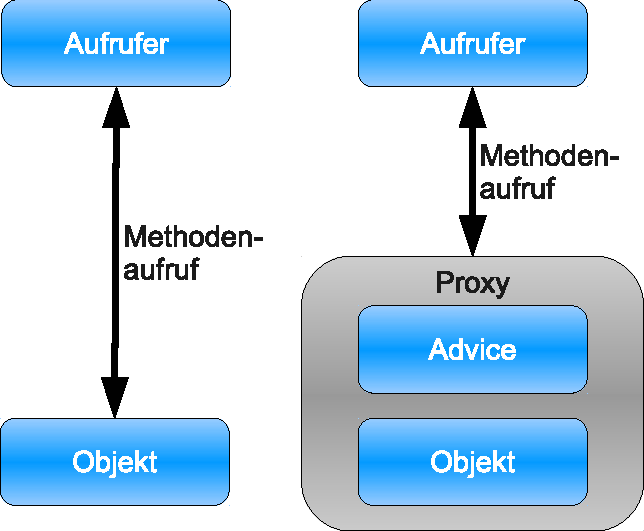
\includegraphics[width=0.6\linewidth]{images/proxy}}
	\caption{Verwendung eines AOP Proxy für einen Methodenaufruf}
	\label{ill:aopproxy}
\end{figure}
 
\subsubsection{Weitere Merkmale}
Neben den oben vorgestellten Eigenschaften der Dependency Injection
und aspektorientierten Programmierung unterstützt das Spring Framework eine
Reihe weiterer Technologien und Architekturprinzipien
(entnommen aus \cite{spring:reference}):

\begin{description}
\item[Convention Over Configuration] Viele Anwendungsframeworks \\ auf der Java
Plattform sind sehr flexibel gestaltet und benötigen deshalb umfangreiche und
detaillierte Konfigurationseinstellungen, um bei der Entwicklung einer konkreten
Anwendung verwendet werden zu können. Im Gegensatz dazu sieht Convention Over
Configuration vor, dass der Konfigurationsaufwand durch sinnvolle
Standardeinstellungen und Namenskonventionen so gering wie möglich gehalten
werden kann. Es ist ein bei Entwicklern inzwischen sehr beliebtes Prinzip.
Deshalb soll auch in den hier vorgestellten Implementierungen wenn möglich nach
dem Convention Over Configuration Prinzip vorgegangen werden.
\item[Security Modul] Spring Security ist ein Unterprojekt
des Spring Framework für die Absicherung von Anwendungen, die auf dem Spring
Framework basieren. Die verschiedenen Merkmale und Funktionen von Spring
Security werden in Abschnitt \ref{service:security} näher vorgestellt.
\item[Vereinfachte ORM Nutzung] Das Spring Framework bietet außerdem Klassen an,
die die Nutzung von verschiedenen \ac{ORM} Frameworks vereinheitlichen und
vereinfachen. \ac{ORM} Technologien werden in Kapitel \ref{subsec:orm} genauer
behandelt.
\item[Remote Anbindung] Durch den Dependency Injection Container kann das Spring
Framework die Arbeit mit verschiedenen \ac{RPC} Protokollen
deutlich vereinfachen. Eine Möglichkeit für die Verwendung der bereitgestellten
Klassen ist in Abschnitt \ref{subsec:rmi} zu finden.
\item[Web MVC Framework] Eine Weboberfläche ist eine Möglichkeit für die
Darstellung im Presentation Layer einer Anwendung. Hierfür bietet das Spring
Framework ein Modul, das auf Basis der anderen Spring Framework
Funktionalitäten die Erstellung von Webapplikationen in Java unterstützt.
\end{description}

\section{Remote Procedure Call}\label{sec:rpc}
Ein \ac{RPC}, oder auch entfernter Prozeduraufruf, erlaubt die Ausführung von
Prozeduren und Methoden in einem anderen Adressraum. Die Adressräume können sich
auch auf physikalisch unterschiedlichen Systemen befinden, die über ein Netzwerk
verbunden sind. Die Grundidee des \ac{RPC} geht auf \cite{rfc707} vom 14. Januar
1976 zurück. Darin wird die Notwendigkeit eines generischen Protokolls beschrieben,
das den Aufruf von Operationen mit mehr als einem Parameter auf einem anderen
Host des ARPANET\footnote{Anfang 1976 bestand das ARPANET aus 75 Host
Systemen} ermöglicht.

Das \ac{RPC} Modell selbst beschreibt Sun Microsystems im Jahr 1988 in
\cite{rfc1057} und \cite{rfc1831}. So soll ein \ac{RPC} ähnlich wie ein lokaler
Methodenaufruf arbeiten. Bei einem lokalen Aufruf stellt der Aufrufer eine Liste
von Argumenten zur Verfügung und übergibt diese an eine Methode oder Funktion.
Anschließend übernimmt diese den weiteren Kontrollfluss des Programms und kehrt
am Ende wieder mit einem Ergebnis zum Aufrufer zurück.

Im Gegensatz dazu erstreckt sich der Aufruf eines \ac{RPC} über
zwei Prozesse, nämlich den Aufrufenden- und den Serverprozess. Der aufrufende
Prozess (Client) sendet eine Nachricht mit den Aufrufparametern an den
Serverprozess (Server) und wartet auf eine Antwortnachricht. Der Server befindet
sich bis dahin im wartenden Zustand. Trifft eine Nachricht ein, wird sie gelesen,
die entsprechenden Operationen ausgeführt und das Ergebnis zurückgesendet. Bei
einem synchronen \ac{RPC} handelt es sich somit um eine direkte Client-Server
Kommunikation. Das \ac{RPC} Modell schreibt nicht vor, dass die Ausführung
synchron erfolgen muss, auch eine asynchrone Ausführung ist möglich. Dadurch
muss der Client nach dem Aufruf des \ac{RPC} nicht warten, bis die Antwort des Servers
eintrifft, sondern kann andere Aufgaben ausführen. Liegt das Ergebnis vor, wird
der Client darüber informiert\footnote{Beispiel einer asynchronen
Kommunikation ist der Empfang und Versand von E-Mails}. Im weiteren Verlauf
dieser Arbeit sollen synchrone \ac{RPC} Protokolle behandelt werden.

\subsection{Herausforderungen}
Im Vergleich zu lokalen Methodenaufrufen sind bei entfernten Methodenaufrufen
verschiedene zusätzliche Faktoren zu berücksichtigen:

\begin{description}
\item[Fehlerquellen] Neben Fehlern, die auch bei lokalen Methodenaufrufen
auftreten können, muss sich der Client mit Problemen befassen, die durch die
bei einem \ac{RPC} notwendige Kommunikation und die Ausführung in zwei
getrennten Ausführungsumgebungen auftreten können. So kann es vorkommen, dass der
Serverprozess gar nicht oder in einer unerwarteten Form antwortet, die
Verbindung während der Kommunikation abbricht, oder das Netzwerk nicht
erreichbar ist.
\item[Kommunikationsoverhead] Für die Kommunikation mit einem anderen Prozess
muss eine Nachricht in eine Form gebracht werden, die über das Netzwerk
übertragen werden kann. Nach der Übertragung müssen die empfangenen Daten dann
auf der Serverseite so konvertiert werden, dass der Serverprozess damit arbeiten
kann. All diese Schritte sind mit zusätzlichem Aufwand verbunden weshalb ein
\ac{RPC} deutlich langsamer als ein lokaler Methodenaufruf ist.
\item[Kein globaler Zustand] Da der Serverprozess nicht auf den Adressraum des
Client zugreifen kann, hat er keine direkten Informationen über dessen globalen
Zustand. Für die Bereitstellung der benötigten Informationen wird zwischen
\emph{zustandsloser} und \emph{zustandsbehafteter} Kommunikation unterschieden.
Bei einer zustandslosen Kommunikation muss der Client mit jedem \ac{RPC}
sämtliche Informationen übertragen, die der Serverprozess benötigt, um diesen
bearbeiten zu können. Bei einer zustandsbehafteten Kommunikation authentifiziert
sich ein Client zu Beginn bei dem Serverprozess. Die dabei gewonnene
Information kann bei nachfolgenden Anfragen dazu verwendet werden, den Client
eindeutig zu identifizieren. Dadurch kann ein serverseitiger globaler Zustand für
alle Anfragen eines Client geschaffen werden.
\item[Beschreibung] Die von einem Server bereitgestellten Methoden müssen in
einer für den Client verständlichen Form beschrieben werden. Für diesen
Zweck bieten einige \ac{RPC} Protokolle jeweils eine eigene \ac{IDL} an.
\item[Lokalisierung] Neben der Beschreibung der bereitgestellten Methoden
muss ein Client auch wissen, wo und wie diese zu finden sind. Oft werden
hierfür Namensdienste verwendet, wo einem Client über einen ihm bekannten Namen
die notwendigen Informationen bereitgestellt werden, mit welchen er sich
dann mit dem gewünschten Server verbinden kann.
\item[Authentifizierung] Werden entfernte Methodenaufrufe über ein unsicheres
Netzwerk übertragen, muss sich ein Client gegenüber dem Server authentifizieren.
\end{description}

\subsection{Methoden- und Funktionsaufrufe}
Das \ac{RPC} Prinzip wurde erstmals zu einem Zeitpunkt beschrieben, als die
prozedurale Programmierung das vorherrschende Programmierparadigma war. Die zu
übertragenden Informationen bestanden dabei aus Prozedurname und den Parametern.
Durch die Entwicklung hin zur objektorientierten Programmierung änderten sich
auch die Anforderungen der bei einem \ac{RPC} zu übertragenenen Informationen.
Bei einem entfernten Methodenaufruf ist es notwendig, neben dem Methodennamen
und den Paramtern auch das Objekt zu identifizieren bzw. zu übertragen, auf dem
diese Methode ausgeführt werden soll. Die Probleme, die sich dabei für ein \ac{RPC}
Protokoll ergeben, das objektorientiert, transparent und bidirektional arbeiten
soll, werden in \cite{waldo:1994} näher erläutert und sollen hier nicht in
allgemeiner Form behandelt werden. Herausforderungen einzelner Implementierungen
werden bei der Vorstellung des jeweiligen \ac{RPC} Protokolls in Kapitel
\ref{sec:protocolhandler} näher erläutert.

\subsection{Webservices}
Eine besondere Form eines \ac{RPC} sind Webservices. Formell wurden
Webservices von einer Arbeitsgruppe des W3C\footnote{\url{http://www.w3.org}}
Konsortium wie folgt definiert (Übersetzung frei nach \cite{mcCabe:2004}
Abschnitt 1.4):

Ein Webservice ist ein Softwaresystem, das die Maschine zu
Maschine-Kommunikation unterschiedlicher Plattformen unterstützt. Die Schnittstelle ist in einem
maschinenlesbaren Format beschrieben (speziell in der \ac{WSDL}). Andere Systeme
kommunizieren mit einem Webservice über diese Schnittstellenbeschreibung unter
der Verwendung von SOAP\footnote{SOAP stand früher für die Abkürzung \emph{Simple
Object Access Protocol}. Da die Spezifikation in der Version 1.2 letzendlich aber
alles andere als "`Simple"' ausfiel wurde entschieden SOAP als Namen und nicht
mehr als Akronym zu verwenden} Nachrichten, die HTTP als Übertragungsprotokoll
und XML sowie andere Web Standards für den Austausch verwenden.

Die Webservice Technologien um SOAP und die verschiedenen Erweiterungen haben
sich zu einem sehr komplexen Themengebiet entwickelt und sollen im Rahmen dieser
Arbeit nicht weiter behandelt werden. Ein anderer Webservice Ansatz in Form von
\ac{REST}\footnote{Für eine genauere Einordnung siehe \cite{mcCabe:2004}
Abschnitt 3.1.3}, der momentan vor allem in Webanwendungen wachsenden Zuspruch
findet, wird in Abschnitt \ref{subsec:rest} vorgestellt. Das XML-RPC Protokoll,
das eine Art Vorgänger von SOAP darstellt und lediglich einfache
Prozeduraufrufe erlaubt, wird in Abschnitt \ref{subsec:xmlrpc} beschrieben.

\section{Austauschformate}\label{sec:datatransfer}
Um Daten über ein Netzwerk übertragen oder in einer Datei speichern zu können,
müssen sie in einer Form vorliegen, die die Übertragung und Wiederherstellung
dieser Daten verlustfrei ermöglicht. Die Konvertierung in ein entsprechendes Format wird
\emph{Serialisierung} genannt, der umgekehrte Fall \emph{Deserialisierung}. Dabei
können die gleichen Daten in verschiedenen Formaten dargestellt werden, von
denen einige in folgenden Abschnitten beschrieben werden.

\subsection{Binärformate}
Eine direkte Möglichkeit der Übertragung ist es, die vorhandenen Daten, so wie
sie im lokalen Adressraum der Anwendung vorliegen, in binärer Form zu übertragen.
Der dafür notwendige Aufwand ist äußerst gering und eine Serialisierung der Daten
nicht notwendig. Ein direktes Abbild des Speichers kann aber oft nur von der
Programmiersprache, in der die Anwendung entwickelt wurde, interpretiert werden.
Deshalb sind native binäre Austauschformate sehr anwendungsspezifisch und nicht
portabel.

Allgemeine binäre Austauschformate, mit denen sich beliebige Daten portabel
übertragen lassen, sind häufig mit einer komplexen Spezifikation verbunden, da
neben der Strukturierung der Daten auch festgelegt werden muss, in welcher Form
diese kodiert werden. Dadurch kann der notwendige Serialisierungs- und
Deserialisierungsaufwand dann deutlich höher ausfallen.

\subsection{Extended Markup Language}\label{subsec:xml}
Bei dem immer größer werdenden Umfang vernetzter Informationen in verschiedenen
Formaten wird die digitale Erfassung, Kategorisierung und Durchsuchung dieser
Daten deutlich erschwert. Viele Austauschformate berücksichtigen auch nicht die
Anforderungen, die sich an Portabilität und Interoperabilität ergeben, wenn die
Daten in einem heterogenen Netzwerk verwendet werden sollen. Deshalb wurden
verschieden Auszeichnungssprachen (\emph{Markup Language}) entwickelt, die eine
allgemeine textuelle Darstellung strukturierter Informationen erlauben. Der erste
Standard für die Definition von Auszeichnungssprachen wurde im Jahr 1986 in Form
der \ac{SGML} \cite{iso8879} verabschiedet. Aufgrund seiner hohen
Flexibilität ist \ac{SGML} aber auch sehr komplex.

Eine durch \ac{SGML} beschrieben Auszeichnungssprache ist die \ac{HTML}
(aktuell ist die Version 4.01, siehe \cite{Jacobs:1999}). Sie bildet die Grundlage des
heutigen World Wide Web. Dabei wurde versucht \ac{HTML} für Entwickler einfach
zugänglich zu machen und durch eine einfachere Syntax die Komplexität der
Webbrowser möglichst gering zu halten.

Neben der Weiterentwicklung von \ac{HTML} wurde gleichzeitig daran gearbeitet,
eine allgemeine Auszeichnungssprache zu entwerfen, die einen Großteil der
Möglichkeiten der \ac{SGML} bietet, aber einfacher zu benutzen ist. Als
Ergebnis veröffentlichte eine Arbeitsgruppe des W3C Konsortiums im Februar 1998
den ersten Vorschlag der \ac{XML} (aktuell ist die Version 5, siehe
\cite{bray:2008}). \ac{XML} stellt eine Untermenge der \ac{SGML} dar, deckt aber
trotzdem einen Großteil der \ac{SGML} Anwendungsfälle ab und soll in erster Linie
dem portablen Datenaustausch im World Wide Web dienen. Durch das standardisierte
Format ist grundsätzlich jeder Teilnehmer in der Lage ein \ac{XML} Dokument zu
lesen. Mit \ac{XML} lassen sich aber nicht nur Online Inhalte sondern auch jede
andere Form von Daten strukturieren, übertragen und speichern. Viele aktuelle
Dateiformate setzen deshalb auf \ac{XML}, und auch für die Konfiguration von
Anwendungen hat sich \ac{XML} inzwischen als de facto Standard durchgesetzt.
Durch entsprechende Transformationsregeln ist es oft problemlos möglich,
zwischen verschiedenen \ac{XML} Formaten zu konvertieren.

Listing \ref{lst:xmlexample} zeigt ein Beispiel für ein \ac{XML} Dokument,
angelehnt an das JavaBean Beispiel aus Kapitel \ref{subsec:javabeans}.

\pagebreak
\lstset{language=XML}
\lstinputlisting[caption=Beispiel eines XML Dokuments, label=lst:xmlexample]
{sources/xml_example.xml}

\subsection{JavaScript Object Notation}
\ac{JSON} ist ein Textformat für die Serialisierung strukturierter Daten
\cite{rfc4627}. Es handelt sich dabei um eine Untermenge der Syntaxdefinition der
ECMAScript Programmiersprache. \ac{JSON} definiert die primitiven
Typen \emph{String}, \emph{Number}, \emph{Boolean}, \emph{Null} und die
zusammengesetzten Typen \emph{Object} und \emph{Array}. In ECMAScript entspricht
der Typ \emph{Object} einem assoziativen Array mit einem eindeutigen String als
Schlüssel. Ein Array ist eine geordnete Menge, die aus keinem oder mehreren
beliebigen primitiven Typen, Objekten oder Arrays bestehen kann.

Vor allem in Anwendungen, die in ECMAScript Dialekten wie \emph{JavaScript} oder
\emph{ActionScript} (Flash) entwickelt werden, ist \ac{JSON} als Austauschformat
äußerst beliebt. Dies ist vor allem darauf zurückzuführen, dass es sich bei
\ac{JSON} Daten um Quelltext handelt, der direkt interpretiert werden kann und
als Ergebnis die entsprechenden Objekte zurückliefert. Aber auch für viele andere
Programmiersprachen existieren inzwischen \ac{JSON} Parser und Generatoren, da
eine kompakte Darstellung möglich ist und die Serialisierung und Deserialisierung
mit deutlich weniger Aufwand verbunden ist, als es beispielsweise bei XML der
Fall ist.

ECMAScript ist eine dynamisch typisierte Programmiersprache, weshalb es auch für
\ac{JSON} keine Schemadefinition gibt. Es handelt sich aber um eine sichere
Untermenge von ECMAScript. Das heißt, dass es sich bei validem \ac{JSON} zwar um
ausführbaren Quelltext handelt, dieser aber nur die oben beschriebenen
Datenelemente enthalten kann. Zuweisungen, Funktionsdeklarationen und
Funktionsaufrufe sind nicht möglich.

\lstset{language=Java}
\lstinputlisting[caption=JSON Beispiel, title=Beispiel einer Benutzerliste in
JSON] {sources/json_example.js}

\subsection{Äquivalenzen zu assoziativen Arrays}\label{subsec:assocequ}
Auch \ac{JSON} und \ac{XML} lassen sich in deserialisierter Form als assoziatives
Array darstellen. Die folgende Beispiele sollen die Äquivalenz von einem
JavaBean, einer Java HashMap und der entsprechenden serialisierten Form in
\ac{XML} und \ac{JSON} aufzeigen.

Als Grundlage wird das JavaBean Beispiel aus Kapitel \ref{subsec:javabeans}
verwendet. Der Java Quelltextauszug in Listing \ref{lst:javaequ} instanziiert
ein User JavaBean und eine Java Map mit identischen Datenelementen:

\lstset{language=Java}
\begin{lstlisting}[caption=JavaBean und äquivalente Java Map, label=lst:javaequ]
// User JavaBean
User userBean = new User();
userBean.setUsername("User");
// MD5(secret) = 5ebe2294ecd0e0f08eab7690d2a6ee69
userBean.setPassword("5ebe2294ecd0e0f08eab7690d2a6ee69");
	
// Java Map
Map<String, Object> userMap = new HashMap<String, Object>();
userMap.put("username", "User");
userMap.put("password", "5ebe2294ecd0e0f08eab7690d2a6ee69");
\end{lstlisting}

Listing \ref{lst:xmlequ} zeigt die nach \ac{XML} serialisierte Darstellung dieser
Daten. Durch die hohe Flexibilität von \ac{XML} wäre auch eine anderer Aufbau
möglich.

\lstset{language=xml}
\begin{lstlisting}[caption=XML Darstellung eines JavaBean, label=lst:xmlequ]
<?xml version="1.0" encoding="UTF-8"?>
<user>
	<username>User</username>
	<password>5ebe2294ecd0e0f08eab7690d2a6ee69</password>
</user>
\end{lstlisting}
\pagebreak
Das folgenden Listing \ref{lst:jsonequ} zeigt eine äquivalente Darstellung
dieses Beans in \ac{JSON}:

\lstset{language=Java}
\begin{lstlisting}[caption=JSON Darstellung eines JavaBean, label=lst:jsonequ]
{ 
	"username" : "User",
	"password" : "5ebe2294ecd0e0f08eab7690d2a6ee69"
}
\end{lstlisting}

Die Äquivalenz von JavaBeans und assoziativen Arrays nimmt in Kapitel
\ref{sec:serviceengine} eine wichtige Rolle für die Konvertierung von
Methodenparametern ein. In Kapitel \ref{subsec:rest} werden für Daten
in Form eines JavaBean unter anderem Darstellungsmöglichkeiten für \ac{XML} und
\ac{JSON} implementiert.